\section{Results}
\label{sec:results}

\subsection{Completed Evaluation and Primary Comparison}
\label{sec:results-primary}

The released record contains all 30 primary replicas, 12 TRAIN-label control runs, and 12 positive-control runs, with no recorded replica failures. These groups are not pooled. The primary results concern the harmonic-feature TQK--SVC benchmark described in Section~\ref{sec:methods-scope}, not the network State8--AFSE--MLP demonstrator. All statistics in Tables~\ref{tab:main-performance} and~\ref{tab:paired-results} retain the canonical reporting conventions. The new descriptive and association analyses below use published scores and diagnostics, without new model fits or TEST predictions~\cite{aqse2026canonical}.

% Generated from canonical aggregate_statistics.json. Do not hand-edit numbers.
\begin{table*}[t]
\caption{Held-out performance across 30 primary replicas. Brackets are the canonical 95\% percentile-bootstrap intervals for the mean; SD is the sample standard deviation across replicas.}
\label{tab:main-performance}
\centering
\small
\setlength{\tabcolsep}{5pt}
\begin{tabular}{lcccccc}
\toprule
& \multicolumn{3}{c}{Balanced accuracy} & \multicolumn{3}{c}{Macro-F1} \\
\cmidrule(lr){2-4}\cmidrule(lr){5-7}
Method & Mean & 95\% interval & SD & Mean & 95\% interval & SD \\
\midrule
TQK & 0.9528 & [0.9333, 0.9708] & 0.0544 & 0.9523 & [0.9312, 0.9707] & 0.0556 \\
RBF-SVC & 0.9569 & [0.9444, 0.9694] & 0.0371 & 0.9568 & [0.9428, 0.9694] & 0.0373 \\
MLP-11 & 0.9750 & [0.9639, 0.9861] & 0.0321 & 0.9749 & [0.9624, 0.9861] & 0.0322 \\
RFF-256 & 0.9472 & [0.9292, 0.9653] & 0.0512 & 0.9468 & [0.9282, 0.9651] & 0.0519 \\
Gradient boosting & 0.9806 & [0.9708, 0.9903] & 0.0284 & 0.9805 & [0.9707, 0.9902] & 0.0285 \\
\bottomrule
\end{tabular}
\end{table*}

% Canonical unadjusted inference; W/T/L is a descriptive post hoc count.
\begin{table*}[t]
\caption{Paired TEST comparisons. Differences are TQK minus baseline. Intervals and unadjusted two-sided Pratt--Wilcoxon $p$-values are canonical. W/T/L denotes balanced-accuracy wins, ties, and losses with tolerance $10^{-12}$; this tolerance is not used to recompute the canonical tests.}
\label{tab:paired-results}
\centering
\small
\setlength{\tabcolsep}{4.5pt}
\begin{tabular}{lccccl}
\toprule
Baseline & Metric & Mean difference & 95\% interval & $p$ & BA W/T/L \\
\midrule
RBF-SVC (primary) & BA & -0.0042 & [-0.0222, +0.0125] & 0.9328 & 10/10/10 \\
 & Macro-F1 & -0.0045 & [-0.0226, +0.0125] & 0.9162 &  \\
\addlinespace[2pt]
MLP-11 & BA & -0.0222 & [-0.0444, -0.0014] & 0.0311 & 4/13/13 \\
 & Macro-F1 & -0.0226 & [-0.0442, -0.0027] & 0.0731 &  \\
\addlinespace[2pt]
RFF-256 & BA & +0.0056 & [-0.0194, +0.0306] & 0.5560 & 11/10/9 \\
 & Macro-F1 & +0.0055 & [-0.0183, +0.0311] & 0.5014 &  \\
\addlinespace[2pt]
Gradient boosting & BA & -0.0278 & [-0.0486, -0.0083] & 0.0166 & 5/11/14 \\
 & Macro-F1 & -0.0282 & [-0.0497, -0.0083] & 0.0431 &  \\
\bottomrule
\end{tabular}
\end{table*}


The mean TEST balanced accuracy was 0.9528 for TQK and 0.9569 for the primary RBF-SVC baseline. The paired mean difference was $-0.0042$, or $-0.42$ percentage points, with a 95\% bootstrap interval of $[-0.0222,0.0125]$. The two-sided Pratt--Wilcoxon statistic was 201.0, with $p=0.9328$. Neither condition of the preregistered predictive-advantage criterion was met. This result does not establish equivalence: no equivalence margin was specified, and the interval includes both positive and negative differences.

TQK exceeded RBF in ten replicas, tied it in ten, and fell below it in ten. These descriptive counts treat absolute score differences no larger than $10^{-12}$ as ties. The canonical bootstrap and Wilcoxon calculations retain the original unrounded values. This distinction matters for one TQK--MLP pair that differs only at floating-point roundoff; it does not alter the primary comparison.

\begin{figure}[t]
\centering
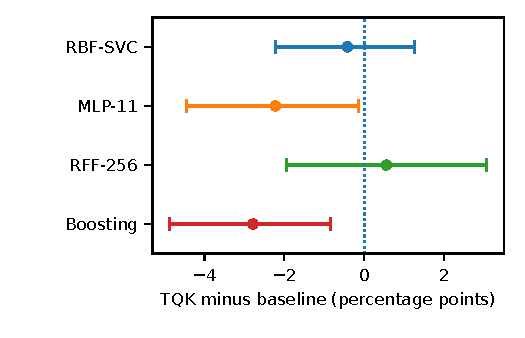
\includegraphics[width=\columnwidth]{figures/results_paired_delta.pdf}
\caption{Primary-study paired balanced-accuracy differences, expressed in percentage points. Points and bars are the canonical mean differences and 95\% bootstrap intervals. Only the RBF-SVC balanced-accuracy comparison defines the preregistered primary criterion. The other comparisons are secondary.}
\label{fig:results-paired}
\end{figure}

\subsection{Secondary Metrics and Between-Replica Variation}
\label{sec:results-variation}

The largest mean balanced accuracy was 0.9806 for gradient boosting, followed by 0.9750 for MLP-11, 0.9569 for RBF-SVC, 0.9528 for TQK, and 0.9472 for RFF-256. Macro-F1 had the same ordering. For TQK versus RBF, the macro-F1 difference was $-0.0045$ with interval $[-0.0226,0.0125]$ and $p=0.9162$.

The secondary TQK-minus-MLP and TQK-minus-boosting balanced-accuracy differences were $-0.0222$ and $-0.0278$, with unadjusted $p=0.0311$ and $p=0.0166$, respectively. TQK minus RFF was $0.0056$, with interval $[-0.0194,0.0306]$ and $p=0.5560$. The two negative secondary intervals are not simultaneous confidence intervals. For macro-F1, the corresponding TQK--MLP and TQK--boosting unadjusted $p$-values were 0.0731 and 0.0431.

As a post-hoc multiplicity sensitivity check, applying Holm's procedure~\cite{holm1979multiple} to all four balanced-accuracy comparisons gives adjusted $p=0.0664$ for boosting and $p=0.0932$ for MLP. Restricting that family to the three secondary comparisons instead gives 0.0498 and 0.0621. Neither family definition was preregistered. We retain the raw secondary results and disclose this dependence on the testing family rather than using a retrospective family choice to make a confirmatory claim.

\begin{figure}[t]
\centering
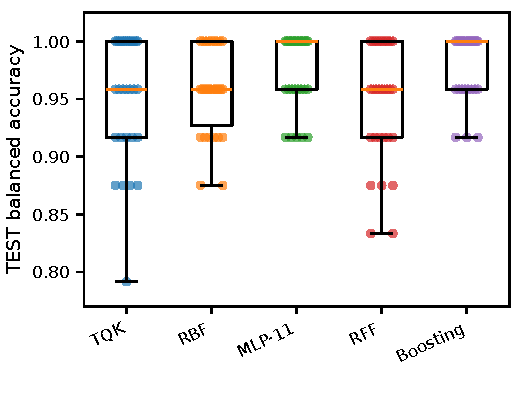
\includegraphics[width=\columnwidth]{figures/results_performance.pdf}
\caption{TEST balanced accuracy in all 30 primary replicas per method. Boxes show medians and interquartile ranges; whiskers extend to observations within 1.5 interquartile ranges. Every observation is plotted, including those outside the whiskers. Horizontal spreading separates tied scores and does not change their values.}
\label{fig:results-performance}
\end{figure}

TQK had the largest observed between-replica standard deviation, 0.0544, compared with 0.0371 for RBF and 0.0284 for boosting. It reached balanced accuracy 1 in 13 of 30 replicas but fell below 0.90 in five. The corresponding below-0.90 counts were two for RBF, zero for MLP, five for RFF, and zero for boosting. The minimum TQK score was 0.7917 in replica 15. This replica is retained in every reported aggregate. Figure~\ref{fig:results-performance} shows the score distributions; no test of equal variances is used. These descriptive differences cannot isolate dataset, split, or initialization effects because those sources of randomness vary together.

\subsection{Kernel Geometry and Checkpoint Selection}
\label{sec:results-kernel}

The primary archive contains 330 TRAIN-kernel diagnostic records: the initial checkpoint and ten accepted updates in each of 30 replicas. VALIDATION selected checkpoint 0 in 19 replicas and an updated checkpoint in 11. The nonzero selections were checkpoint 1 once, checkpoint 2 four times, checkpoint 3 once, checkpoint 4 twice, checkpoint 5 once, and checkpoint 7 twice. No selected checkpoint was chosen from TEST performance.

Across the selected $72\times72$ uncentered Gram matrices, the mean effective rank was 28.8241, with a 95\% interval of $[28.0758,29.5220]$. The mean largest-eigenvalue share, $c_{\rm spec}$, was 0.2160, with interval $[0.2076,0.2243]$, and the trace was approximately 72. Selected effective ranks ranged from 24.9784 to 32.7250; selected spectral concentrations ranged from 0.1746 to 0.2676. These finite-sample summaries differ from both a rank-one limit and an identity Gram matrix. They do not measure circuit expressivity or establish predictive generalization.

\begin{figure}[t]
\centering
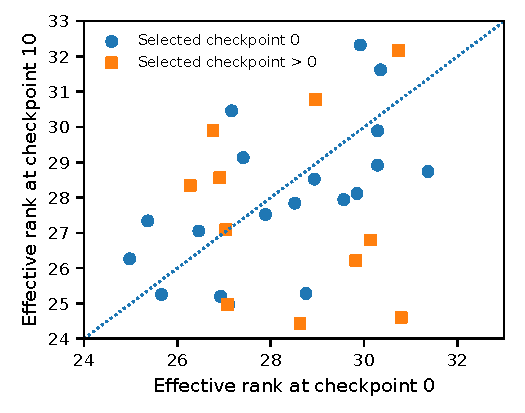
\includegraphics[width=\columnwidth]{figures/results_rank_change.pdf}
\caption{Initial versus checkpoint-10 effective rank for all 30 primary replicas. The dotted line denotes equal rank. Marker shape indicates whether VALIDATION selected the initial or an updated checkpoint; the vertical coordinate always refers to checkpoint 10. This is a comparison of stored kernel diagnostics, not a trained-versus-untrained TEST comparison.}
\label{fig:results-rank-change}
\end{figure}

Comparing checkpoint 10 with checkpoint 0, effective rank increased in 13 replicas and decreased in 17. Its mean change was $-0.4566$, while the mean absolute change was 1.9701; individual changes ranged from $-6.1879$ to $3.2980$. Spectral concentration increased in nine replicas and decreased in 21, with mean change $-0.0096$. Thus optimization changed the recorded spectral summaries without a common direction of effective-rank change (Fig.~\ref{fig:results-rank-change}). The archive does not contain TEST evaluations of the unselected initial models. It therefore cannot estimate the paired predictive effect of QNG relative to a fixed initial kernel. Selecting an updated checkpoint is not a substitute for that comparison.

\subsection{Exploratory Geometry--Performance Associations}
\label{sec:results-correlations}

We examined four post-hoc associations: selected effective rank and spectral concentration against TQK TEST balanced accuracy and against its paired difference from RBF. Each analysis uses one selected diagnostic pair per replica, rather than treating the 330 checkpoints as independent observations. Spearman correlations use average ranks~\cite{spearman1904association}. For this analysis only, balanced accuracies are mapped to their verified integer counts on the $1/24$ grid, avoiding artificial rank distinctions due to floating-point roundoff.

% Exploratory analysis; not part of the preregistered criterion.
\begin{table}[t]
\caption{Post-hoc associations between selected-kernel geometry and TEST performance ($n=30$). $\rho_s$ is Spearman correlation; $p_{\rm MC}$ uses 19,999 random pairings with the add-one correction. All four Holm-adjusted values are 1.}
\label{tab:geometry-associations}
\centering
\small
\setlength{\tabcolsep}{4pt}
\begin{tabular}{llrr}
\toprule
Predictor & Endpoint & $\rho_s$ & $p_{\rm MC}$ \\
\midrule
$r_{\rm eff}$ & TQK BA & +0.154 & 0.410 \\
$r_{\rm eff}$ & $\Delta_{\rm TQK-RBF}$ & +0.069 & 0.712 \\
$c_{\rm spec}$ & TQK BA & -0.140 & 0.451 \\
$c_{\rm spec}$ & $\Delta_{\rm TQK-RBF}$ & -0.093 & 0.625 \\
\bottomrule
\end{tabular}
\end{table}


Two-sided association $p$-values use 19,999 random pairings and the add-one correction~\cite{phipson2010permutation}. The four permutation seeds are 4001001--4001004 in table order. Percentile intervals use 2,000 paired replica resamples with seeds 4002001--4002004. The input extracts, calculations, and interval endpoints are included with the manuscript sources. These procedures were defined during manuscript analysis and do not replace any frozen comparison.

The estimated correlations ranged from $-0.140$ to $0.154$, and the unadjusted permutation $p$-values ranged from 0.410 to 0.712 (Table~\ref{tab:geometry-associations}). All four Holm-adjusted $p$-values were 1.000. The intervals were broad. For example, effective rank versus TQK balanced accuracy had $\rho_s=0.154$ and interval $[-0.215,0.501]$. The observed selected-kernel summaries therefore do not resolve a monotonic association with performance in these 30 replicas. This does not exclude weaker, nonlinear, or task-dependent relationships.

\subsection{Control Results}
\label{sec:results-controls}

Table~\ref{tab:control-results} reports the two controls separately. Under TRAIN-label permutation, mean balanced accuracy was 0.6146 for TQK and 0.6271 for RBF. Their canonical intervals excluded 0.5. The intervals for MLP, RFF, and boosting included 0.5. The prespecified chance-compatibility check was therefore not met for the two validation-selected kernel methods. Inclusion of 0.5 for the other methods is not evidence of equivalence to chance.

% Exact control-summary extract, no new control evaluation.
\begin{table}[t]
\caption{Control balanced accuracy. Each cell gives the canonical mean and 95\% bootstrap interval. The negative-control intervals condition on one shared dataset.}
\label{tab:control-results}
\centering
\footnotesize
\setlength{\tabcolsep}{3pt}
\renewcommand{\arraystretch}{1.15}
\begin{tabular}{lcc}
\toprule
Method & TRAIN-label control & Positive control \\
\midrule
TQK & \shortstack{0.6146\\{}[0.5333, 0.6958]} & \shortstack{0.9813\\{}[0.9625, 0.9958]} \\
RBF-SVC & \shortstack{0.6271\\{}[0.5479, 0.7083]} & \shortstack{0.9792\\{}[0.9646, 0.9917]} \\
MLP-11 & \shortstack{0.5521\\{}[0.4750, 0.6292]} & \shortstack{0.9708\\{}[0.9542, 0.9875]} \\
RFF-256 & \shortstack{0.5104\\{}[0.4417, 0.5792]} & \shortstack{0.9688\\{}[0.9479, 0.9854]} \\
Grad. boosting & \shortstack{0.5354\\{}[0.4792, 0.5855]} & \shortstack{0.9333\\{}[0.9000, 0.9625]} \\
\bottomrule
\end{tabular}
\end{table}


These negative-control intervals describe randomized re-splits and permutations conditional on one teacher dataset. Correct VALIDATION labels remained available for checkpoint and hyperparameter selection. The result is thus a limitation of this TRAIN-label ablation, not an observation from a fully label-null pipeline. The present records do not establish why the two methods remained above chance, or establish TEST leakage.

In the positive control, TQK reached mean balanced accuracy 0.9813 and RBF reached 0.9792. Their paired difference was 0.0021, with interval $[-0.0083,0.0125]$ and $p=1.0000$. Against boosting, the difference was 0.0479, with interval $[0.0208,0.0771]$ and unadjusted $p=0.0117$. That control comparison is distinct from the primary sensor-task criterion. The data were generated by a TQK teacher and enriched for large fidelity contrasts. These results establish neither transfer to physical sensors nor a representation exclusive to the quantum method.

\subsection{Recorded Computation and Reproduction}
\label{sec:results-computation}

The recorded total runtimes of the 30 primary replicas sum to 312.94~s. The median was 10.38~s, with a range of 10.15--11.64~s. Each value includes dataset generation, fitting and selection across all methods, and their TEST evaluation. The repeated runtime field in the method-level CSV must be counted once per replica. It does not support a TQK-versus-classical timing comparison or a hardware-speed claim.

A report-only reconstruction of the ten method--metric summaries and eight paired summaries matched the canonical means, intervals, and signed-rank outputs to a maximum absolute difference of $2.8\times10^{-17}$. Tables retain the canonical values. The additional counts, endpoint geometry summaries, and association tests are identified as descriptive or post hoc. No simulations, quantum-state evaluations, training jobs, or TEST predictions were repeated for this section.
